%!TEX root = ../../main.tex


\begin{figure}[!htb]
\centering
%\hrulefill \\
%\vspace{5pt}
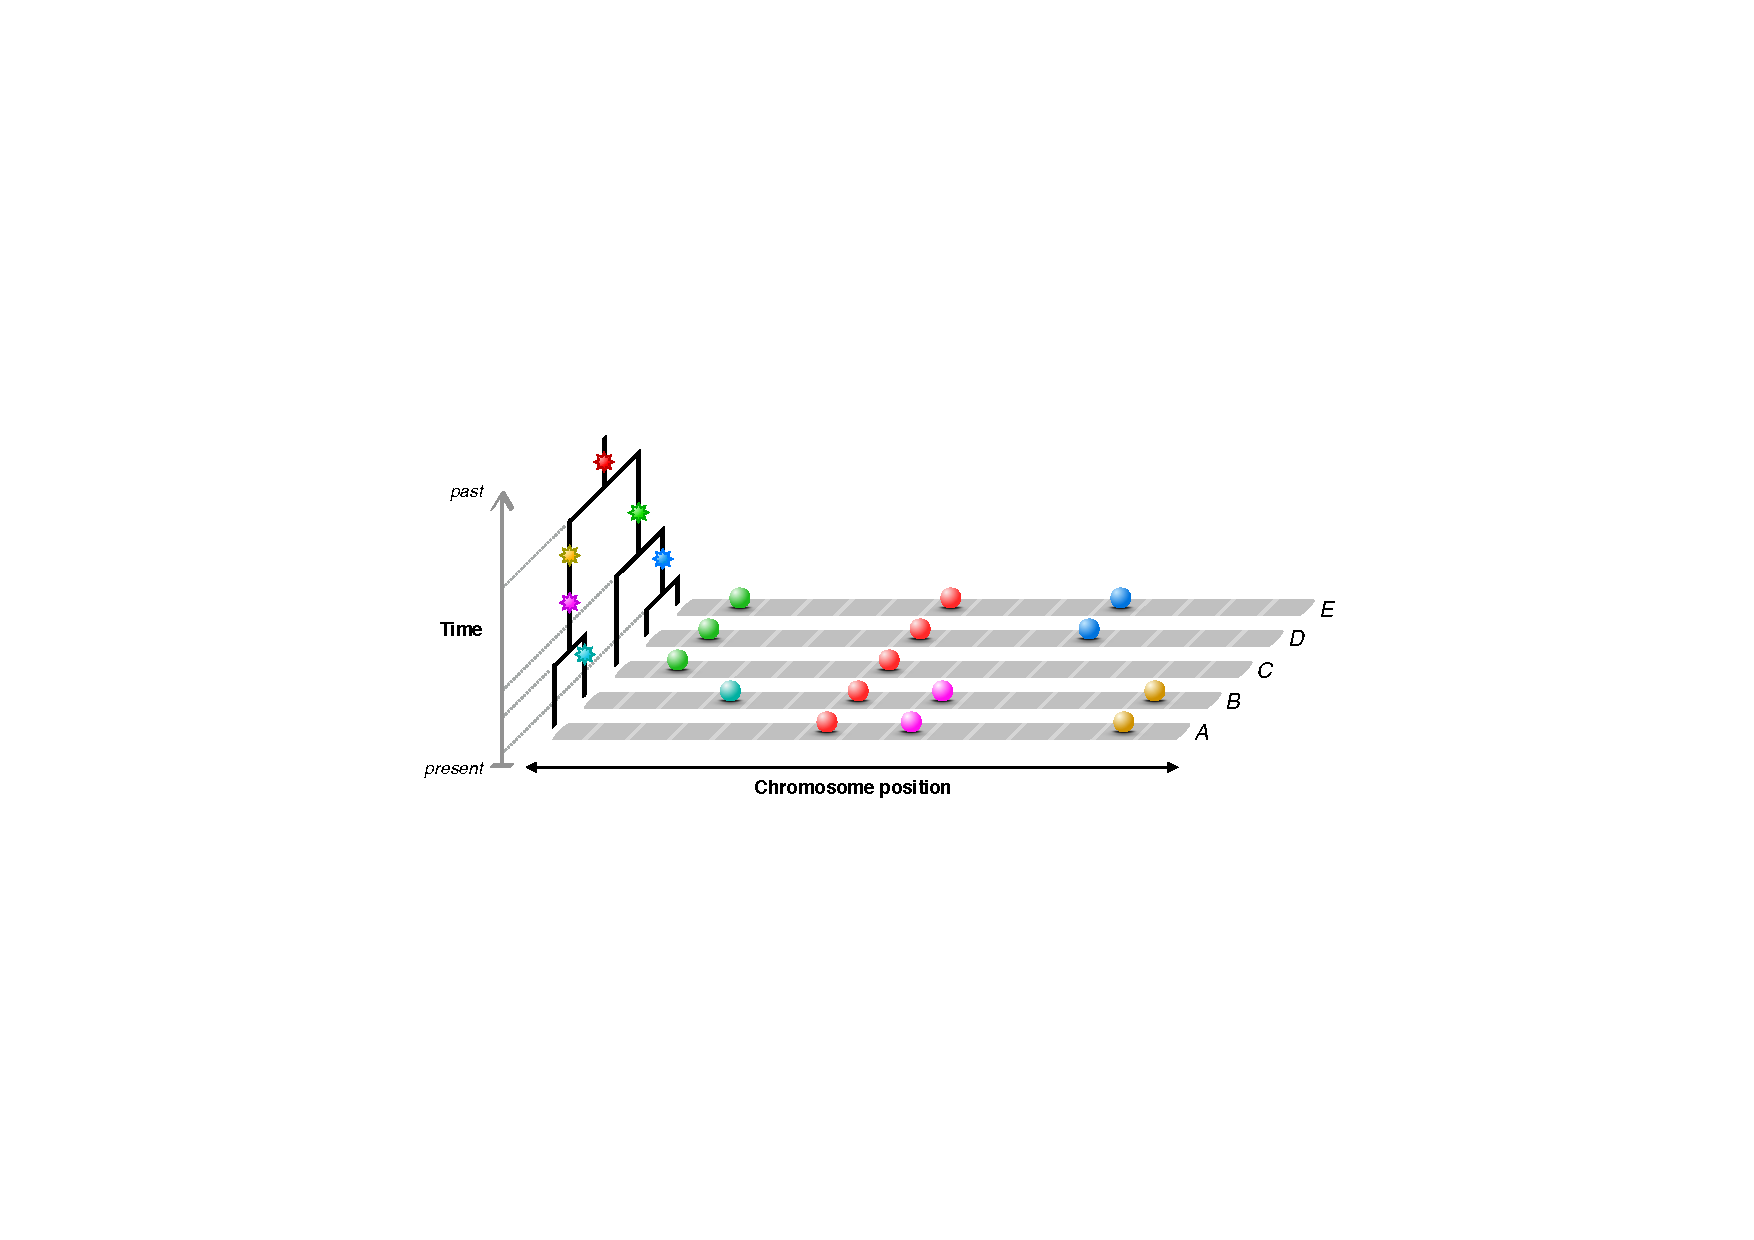
\includegraphics[width=\textwidth]{./img/ch1/info_mutation}
\Caption{Mutation events on a genealogical tree in the coalescent}
{The genealogy of a sample of \n{5} haploid individuals ($A-E$) is shown on the left.
The time of each coalescent event is indicated by a \emph{dotted} line.
Mutation events (\emph{stars}) are placed along the branches of the tree.
Each mutation event alters the allelic state at a random position on the chromosome, giving rise to a new allele, which is inherited by all descendants of the ancestral individual in which the mutation occurred.
Horizontal lanes (\emph{grey}) represent the chromosome sequence of the individuals, on which the derived alleles are depicted as \emph{marbles}; colours correspond to the mutation event from which the alleles derive.}
{fig:info_mutation}
% \vspace{-5pt}
% \hrulefill%
\end{figure}
